% Search for all the places that say "PUT SOMETHING HERE".

\documentclass[11pt]{article}

\usepackage{amsmath,graphicx,textcomp,amssymb,geometry,graphicx,enumerate}
\graphicspath{ {images/} }
\def\Name{Dan Ricciardelli}  % Your name
\def\SID{24568103}  % Your student ID number
\def\Homework{6} % Number of Homework
\def\Session{Fall 2015}

\usepackage[procnames]{listings}
\usepackage{color}

\title{CS189--Fall 2015 --- Homework \Homework\ Solutions}
\author{\Name, SID \SID}
\markboth{CS189--\Session\  Homework \Homework\ \Name}{CS189--\Session\ Homework \Homework\ \Name}
\pagestyle{myheadings}
\date{}

\newenvironment{qparts}{\begin{enumerate}[{(}a{)}]}{\end{enumerate}}
\def\endproofmark{$\Box$}
\newenvironment{proof}{\par{\bf Proof}:}{\endproofmark\smallskip}

\textheight=9in
\textwidth=6.5in
\topmargin=-.75in
\oddsidemargin=0.25in
\evensidemargin=0.25in


\begin{document}
\definecolor{keywords}{RGB}{255,0,90}
\definecolor{comments}{RGB}{0,0,113}
\definecolor{red}{RGB}{160,0,0}
\definecolor{green}{RGB}{0,150,0}
 
\lstset{language=Python, 
        basicstyle=\ttfamily\small, 
        keywordstyle=\color{keywords},
        commentstyle=\color{comments},
        stringstyle=\color{red},
        showstringspaces=false,
        identifierstyle=\color{green},
        procnamekeys={def,class}}
\maketitle

\section*{1. A. Stochastic Gradient Descent Updates, Square Loss}
\textbf{Derivation for Square Loss}

For the stochastic forward pass using square loss, the necessary values to calculate the output layer were
\newline
$ z^{2} = x.W^{1} $ where x is an input training example appended by a bias column.
\newline
$ a^{2} =  tanh(z^{2}) $, which calculates the activation of the hidden layer. In this implementation, we append a bias column of ones to $a^{2}$ here.
\newline
$ z^{3} = a^{2}.W^{2}$, the input to the output layer.
\newline
And, finally, $h_{k}(x) = sigmoid(z^{3}) $, where the loss function is defined as $ J = 0.5 * \sum_{k=1}^{n_{out}} (y_{k} - h_{k}(x))^{2}$
\newline
Using this, we can compute the gradients $\frac{\partial J}{\partial W^{2}}$ and $\frac{\partial J}{\partial W^{1}}$ by repeated application of the chain rule.
\newline
First, we calculate $\frac{\partial J}{\partial W^{2}} = \frac{\partial J}{\partial h_{k}(x)} * \frac{\partial h_{k}(x)}{\partial W^{2}}$
\newline
The derivative of the loss function with respect to the output is $\frac{\partial J}{\partial h_{k}(x)} = -(y - h(x))$.
\newline
Now, $\frac{\partial h_{k}(x)}{\partial W^{2}} = \frac{\partial h_{k}(x)}{\partial z^{3}} * \frac{\partial z^{3}}{\partial W^{2}}$.
\newline
For the first part, $\frac{\partial h_{k}(x)}{\partial z^{3}} = sigmoid'(z^{3}) = (1 - sigmoid(z^{3}))*sigmoid(z^{3})$ and as $ z^{3} = a^{2}.W^{2}$, the second part is computed as $\frac{\partial z^{3}}{\partial W^{2}} = a^{2}.T$
\newline
Putting this together, $\frac{\partial J}{\partial W^{2}} = (a^{2}.T) . [(1 - sigmoid(z^{3})*sigmoid(z^{3}) .* (-(y - h(x)))]$
\newline
Now we can compute $\frac{\partial J}{\partial W^{1}}$ as $\frac{\partial J}{\partial W^{1}} = \frac{\partial J}{\partial h_{k}(x)} * \frac{\partial h_{k}(x)}{\partial z^{3}} * \frac{\partial z^{3}}{\partial W^{1}}$.
\newline
The first two terms in this multiplication we have already computed, and will define as $ delta3 = \frac{\partial J}{\partial h_{k}(x)} * \frac{\partial h_{k}(x)}{\partial z^{3}}$. 
\newline
The final term can be broken into $\frac{\partial z^{3}}{\partial W^{1}} = \frac{\partial z^{3}}{\partial a^{2}} * \frac{\partial a^{2}}{\partial z^{2}} * \frac{\partial z^{2}}{\partial W^{1}}$.
\newline
Now, again, since $ z^{3} = a^{2}.W^{2}$,  $\frac{\partial z^{3}}{\partial a^{2}} = a^{2}.T$. 
\newline
As $ a^{2} =  tanh(z^{2}) $, $\frac{\partial a^{2}}{\partial z^{2}} = 1 - tanh(z^{2})^{2}$.
\newline
Finally, since 
$ z^{2} = x.W^{1} $, the final term is $\frac{\partial z^{2}}{\partial W^{1}} = x.T$.
\newline
Putting this all together, $\frac{\partial z^{3}}{\partial W^{1}} = (x.T) . [(delta3 . (W2.T)) .* (1 - tanh(z^{2})^{2}] $
\newline
These two partial derivatives are sufficient to compute the update during stochastic gradient descent, $ W1 = W1 - \frac{\partial J}{\partial W^{1}}$ and $ W2 = W2 - \frac{\partial J}{\partial W^{2}}$



\newpage
\section*{1. B. Stochastic Gradient Descent Updates, Entropy Loss}
\textbf{Derivation for Entropy Loss}
\newline
The derivation for the gradient descent update using entropy loss is very similar to that for square loss, but the full details are shown here. 
\newline
For the stochastic forward pass using square loss, the necessary values to calculate the output layer were
\newline
$ z^{2} = x.W^{1} $ where x is an input training example appended by a bias column.
\newline
$ a^{2} =  tanh(z^{2}) $, which calculates the activation of the hidden layer. In this implementation, we append a bias column of ones to $a^{2}$ here.
\newline
$ z^{3} = a^{2}.W^{2}$, the input to the output layer.
\newline
And, finally, $h_{k}(x) = sigmoid(z^{3}) $, where the loss function is defined as $ J = - \sum_{k=1}^{n_{out}} [y_{k}*ln(h_{k}(x)) + (1 - y_{k})* ln(1 - h_{k}(x))]$
\newline
Using this, we can compute the gradients $\frac{\partial J}{\partial W^{2}}$ and $\frac{\partial J}{\partial W^{1}}$ by repeated application of the chain rule.
\newline
First, we calculate $\frac{\partial J}{\partial W^{2}} = \frac{\partial J}{\partial h_{k}(x)} * \frac{\partial h_{k}(x)}{\partial W^{2}}$
\newline
The derivative of the loss function with respect to the output is $\frac{\partial J}{\partial h_{k}(x)} = - [\frac{y_{k}}{h_{k}(x)} - \frac{1 - y_{k}}{1-h_{k}(x)}]$.
\newline
Now, $\frac{\partial h_{k}(x)}{\partial W^{2}} = \frac{\partial h_{k}(x)}{\partial z^{3}} * \frac{\partial z^{3}}{\partial W^{2}}$.
\newline
For the first part, $\frac{\partial h_{k}(x)}{\partial z^{3}} = sigmoid'(z^{3}) = (1 - sigmoid(z^{3}))*sigmoid(z^{3})$ and as $ z^{3} = a^{2}.W^{2}$, the second part is computed as $\frac{\partial z^{3}}{\partial W^{2}} = a^{2}.T$
\newline
Putting this together, $\frac{\partial J}{\partial W^{2}} = (a^{2}.T) . [(1 - sigmoid(z^{3})*sigmoid(z^{3}) .* (\frac{y_{k}}{h_{k}(x)} - \frac{1 - y_{k}}{1-h_{k}(x)})]$
\newline
Now we can compute $\frac{\partial J}{\partial W^{1}}$ as $\frac{\partial J}{\partial W^{1}} = \frac{\partial J}{\partial h_{k}(x)} * \frac{\partial h_{k}(x)}{\partial z^{3}} * \frac{\partial z^{3}}{\partial W^{1}}$.
\newline
The first two terms in this multiplication we have already computed, and will define as $ delta3 = \frac{\partial J}{\partial h_{k}(x)} * \frac{\partial h_{k}(x)}{\partial z^{3}}$. 
\newline
The final term can be broken into $\frac{\partial z^{3}}{\partial W^{1}} = \frac{\partial z^{3}}{\partial a^{2}} * \frac{\partial a^{2}}{\partial z^{2}} * \frac{\partial z^{2}}{\partial W^{1}}$.
\newline
Now, again, since $ z^{3} = a^{2}.W^{2}$,  $\frac{\partial z^{3}}{\partial a^{2}} = a^{2}.T$. 
\newline
As $ a^{2} =  tanh(z^{2}) $, $\frac{\partial a^{2}}{\partial z^{2}} = 1 - tanh(z^{2})^{2}$.
\newline
Finally, since 
$ z^{2} = x.W^{1} $, the final term is $\frac{\partial z^{2}}{\partial W^{1}} = x.T$.
\newline
Putting this all together, $\frac{\partial z^{3}}{\partial W^{1}} = (x.T) . [(delta3 . (W2.T)) .* (1 - tanh(z^{2})^{2}] $
\newline
These two partial derivatives are sufficient to compute the update during stochastic gradient descent, $ W1 = W1 - \frac{\partial J}{\partial W^{1}}$ and $ W2 = W2 - \frac{\partial J}{\partial W^{2}}$

\newpage
\section*{2.Neural Net Implementation}
\begin{qparts}
\item \textbf{Hyperparameter tuning}. The learning rate, alpha, and the standard deviation for the weight initialization given mean zero, init scale were both tuned. A good value for alpha was found to be 0.003125 using grid search on a smaller training size, and this proved suitable for the full training set. A good value for init scale was found to be 0.01, and small alterations from this value were not seen to influence the final result significantly. 

\item Final training accuracy on 16 passes through the full training set was found to be 0.95550, with a validation accuracy of 0.96205.

\item Total running time for 16 epochs was 37 minutes and 16 seconds.

\item Plots for training error and classification error are given below. Validation error is plotted by red dashes, training accuracy is shown by green triangles.
\newline
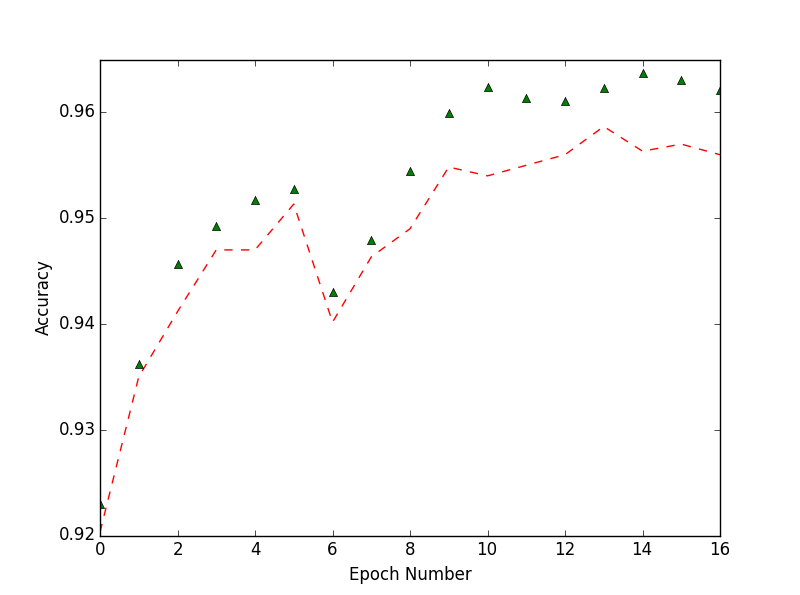
\includegraphics{16_epochs_full_square}

\item Interestingly, I found square error to work better (train faster) than entropy loss. This may have been an error with my implementation of entropy loss backpropogation (or a failure to find properly tuned values of alpha), as square error places too much emphasis on incorrect outputs and entropy loss should train faster than square error in this case.


\end{qparts}
\newpage
\section*{3. Implementation Notes and Kaggle Score}

Using a 'smoothed rectifier unit' as the choice of nonlinearity instead of tanh did speed up training, but did not improve overall results and so is not included here.
\newline
My final Kaggle Score was 0.95560.
\newpage
\section*{4. Code}
\begin{lstlisting}
import random
import csv
import numpy as np
from scipy.io import loadmat
import time
import matplotlib.pyplot as plt

######    Establish some Data Constants    ######
######    for easy access				   ######

image_size = 28*28
image_count = 60000
test_image_count = 10000

######    Load Train Data                  ######

train_data = loadmat("./dataset/train.mat")

train_images = train_data["train_images"]
train_labels = train_data["train_labels"]

train_images = np.swapaxes(train_images, 0, 2)
train_images = np.reshape(train_images, (image_count, image_size))

train_temp = np.zeros((train_images.shape[0], 10))

# Adjust labels for 10 categories
for i in range(train_labels.shape[0]):
	k = train_labels[i]
	train_temp[i][k] = 1

train_labels = train_temp

# Randomly shuffle training data
data = zip(train_images, train_labels)
np.random.shuffle(data)
(X, y) = zip(*data)
train_images = np.array(X)
train_labels = np.array(y)


###### Load Test Data 					   ######

test_data = loadmat("./dataset/test.mat")

test_images = test_data["test_images"]
test_images = np.swapaxes(test_images, 0, 2)
test_images = np.reshape(test_images, (test_image_count, image_size))


######### CLASS DEFINITION ##########

class Neural_Network(object):
	def __init__(self, alpha=0.0001, init_scale=0.01):
		# Hyperparamters
		self.inputLayerSize = 784
		self.hiddenLayerSize = 200
		self.outputLayerSize = 10
		self.alpha = alpha
		self.init_scale = init_scale
		self.W1 = np.array(self.init_scale*np.random.randn(self.inputLayerSize+1, self.hiddenLayerSize))
		self.W2 = np.array(self.init_scale*np.random.randn(self.hiddenLayerSize+1, self.outputLayerSize))

	def forward(self, X):
		# Forward propogate inputs through the network
		# W1 is (785x200)
		# W2 is (201x10)
		N = X.shape[0]
		bias_col = np.ones((N,1))

		# Append bias and multiply to get hidden layer z2

		self.X_bias = np.concatenate((X, bias_col), axis=1)

		# 1x784 x 784x200 = 1x200
		self.z2 = np.dot(self.X_bias, self.W1)
		# append bias

		# Tanh for hidden layer activation
		# 1x200
		self.a2 = self.smooth_rectifier(self.z2)
		self.a2_bias = np.concatenate((self.a2, bias_col), axis=1)
		
		# Multiply to get output layer
		# 1x200 * 200*10 = 1x10
		self.z3 = np.dot(self.a2_bias, self.W2)

		# Sigmoid and return self.outputLayerSize predictions
		# 1x10
		yHat = self.sigmoid(self.z3)

		# Return prediction
		return yHat

	def sigmoid(self, z):
		# Apply Numerically stable sigmoid activation function
		z_new = np.zeros(z.shape)
		for i in range(z.shape[0]):
			for j in range(z.shape[1]):
				x = z[i][j]
				if x >= 0:
					l = np.exp(-x)
					l = 1.0 / (1.0 + l)
				else:
					l = np.exp(x)
					l = l / (1.0 + l)
				z_new[i][j] = l

		return z_new
		# return 1/(1+np.exp(-z))

	def sigmoid_prime(self, z):
		# Apply derivative of sigmoid function
		return self.sigmoid(z)*(1-self.sigmoid(z))

	def tanh(self, z):
		# Apply tanh activation function
		return (np.exp(2*z) - 1.0)/(np.exp(2*z) + 1.0)


	def tanh_prime(self, z):
		# Apply derivative of tanh function
		return 1 - np.multiply(self.tanh(z), self.tanh(z))

	def smooth_rectifier(self, z):
		# Numerically stable smooth rectifier
		z_new = np.ones(z.shape)
		for i in range(z.shape[0]):
			for j in range(z.shape[1]):
				x = z[i][j]
				if x >= 15:
					x = 15
				z_new[i][j] = x

		return np.log(1.0 + np.exp(z_new))

	def smooth_rectifier_prime(self, z):
		# Numerically unstable smooth rectifier prime
		return self.sigmoid(z)

	def coarse_rectifier(self, z):
		# Numerically stable coarse rectifier
		z_new = np.zeros(z.shape)
		for i in range(z.shape[0]):
			for j in range(z.shape[1]):
				x = z[i][j]
				z_new[i][j] = max(0,x)

		return z_new

	def coarse_rectifier_prime(self, z):
		# Numerically stable coarse rectifier derivative
		z_new = np.zeros(z.shape)
		for i in range(z.shape[0]):
			for j in range(z.shape[1]):
				x = z[i][j]
				if (x <= 0):
					x = 0
				else:
					x = 1
				z_new[i][j] = x

		return z_new

	def square_error_cost(self, X, y):
		self.yHat = self.forward(X)
		J = 0.5*(sum((y-self.yHat)**2))
		return J

	def square_error_prop(self, X, y):
		# Compute derivatives with respect to W1 and W2

		# 1x10 
		self.yHat = self.forward(X)

		# Compute dj/dw1
		# delta3 is backprop error at third layer
		# nx10 = nx10 .* nx10
		delta3 = np.multiply((-(y-self.yHat)), self.sigmoid_prime(self.z3))
		# 201x10 = 201xn * nx10
		dJdW2 = np.dot(self.a2_bias.T, delta3)


		# Compute dj/dw2
		# delta2 is backprop error at second layer
		# (nx10 * 10x201) .* nx200
		delta2 = np.multiply(np.dot(delta3, self.W2[0:self.hiddenLayerSize].T), self.smooth_rectifier_prime(self.z2))

		dJdW1 = np.dot(self.X_bias.T, delta2)

		return (dJdW1, dJdW2)

	def entropy_error_prop(self, X, y):
		# Compute derivatives with respect to W1 and W2

		self.yHat = self.forward(X)

		# Compute dj/dw1
		# delta3 is backprop error at third layer
		# 1x10 by 1x10 = 1x10
		cost_grad = np.add(np.divide(y+0.0, self.yHat+0.0), -1*np.divide(1.0-y, 1.0-self.yHat))
		delta3 = np.multiply(cost_grad, self.sigmoid_prime(self.z3))
		#  200x1 * 1x10 = 200x10 
		dJdW2 = np.dot(self.a2_bias.T, delta3)


		# Compute dj/dw2
		# delta2 is backprop error at second layer
		# 1x10 * 10x200 * 1x200
		delta2 = np.multiply(np.dot(delta3, self.W2[0:self.hiddenLayerSize].T), self.smooth_rectifier_prime(self.z2))

		dJdW1 = np.dot(self.X_bias.T, delta2)

		return (dJdW1, dJdW2)


	def stochastic_train(self, X, y, error="square"):
		for k in range(X.shape[0]):
			if ((k % 20000) == 0):	
				print ""
			elif ((k % 1000 ) == 0):
				print ".",

			i = random.choice(range(X.shape[0]))

			############# Prop ############
			# Compute values for each layer
			# Backprop to find Gradient
			Xin = np.reshape(X[i], (1,X[i].shape[0]))
			Yin = np.reshape(y[i], (1,y[i].shape[0]))
			if (error == "square"):
				dJdW1, dJdW2 = self.square_error_prop(Xin, Yin)
			else:
				dJdW1, dJdW2 = self.entropy_error_prop(Xin, Yin)

			######## Gradient Descent #####
			# Update weights

			self.W1 = self.W1 - self.alpha*dJdW1
			self.W2 = self.W2 - self.alpha*dJdW2

		return

	def predict(self, X):
		return self.forward(X)

	def score(self, X, y):
		yHat = np.argmax(self.predict(X), axis=1)

		yVal = np.argmax(y, axis=1)
		score = 0
		for i in range(len(yHat)):

			if (yHat[i] == yVal[i]):
				score += 1.0

		print((score+ 0.0) / X.shape[0])
		print ""
		return (score +0.0) / X.shape[0]

	def cv_score(self, X, y, num_folds=10, error="square"):
		print "CV Training Stochastic Model"
		np.random.seed(1)

		data = zip(X,y)
		np.random.shuffle(data)
		(X, y) = zip(*data)
		X = np.array(X)
		y = np.array(y)
		N = X.shape[0]
		score = 0

		# Train on new cuts
		for i in range(num_folds):

			# Clear weights for training
			self.clear_weights()

			# Establish cuts
			cut0 = int(i*(N/num_folds))
			cut1 = int((i+1)*(N/num_folds))

			# Slice Validation data
			X_val = X[cut0:cut1]
			y_val = y[cut0:cut1]

			# Slice Training data
			X_train = np.concatenate((X[0:cut0],X[cut1:]), axis=0)
			y_train = np.concatenate((y[0:cut0],y[cut1:]), axis=0)

			# Train model
			for i in range(1):
				self.stochastic_train(X_train, y_train, error)

			# Adjust sum scores across each model
			score += self.score(X_val, y_val)

		return (score +0.0) / num_folds

	def cv_plot_score(self, X, y, num_iter=10, error="square"):
		print "CV Training Stochastic Model"
		t = time.clock()
		np.random.seed(1)

		data = zip(X,y)
		np.random.shuffle(data)
		(X, y) = zip(*data)
		X = np.array(X)
		y = np.array(y)
		N = X.shape[0]
		score = 0


		# Clear weights for training
		self.clear_weights()

		# Establish cuts
		cut0 = 0
		cut1 = int(N/10)

		# Slice Validation data
		X_val = X[cut0:cut1]
		y_val = y[cut0:cut1]

		# Slice Training data
		X_train = np.concatenate((X[0:cut0],X[cut1:]), axis=0)
		y_train = np.concatenate((y[0:cut0],y[cut1:]), axis=0)

		# Train model
		val_scores = []
		train_scores = []
		for i in range(num_iter):
			# overfit like crazy?
			self.stochastic_train(X_train, y_train, error)
			val_score = self.score(X_val, y_val)
			train_score = self.score(X_train, y_train)
			val_scores.append(val_score)
			train_scores.append(train_score)
			print("Current run-time for " + str(i+1) + " epochs is " + str(time.clock() -  t))
				
			if (i%2 == 0):
				x = range(len(val_scores))
				plt.plot(x, val_scores, 'r--', x, train_scores, 'g^')
				plt.xlabel("Epoch Number")
				plt.ylabel("Accuracy")
				plt.show()

				# Learning rate decay
				self.alpha = self.alpha*0.75

				# Update predictions .csv
				self.write_prediction(test_images)

		# Adjust sum scores across each model
		score += self.score(X_val, y_val)
		plt.show()

		return score

	def clear_weights(self):
		self.W1 = np.array(self.init_scale*np.random.randn(self.inputLayerSize+1, self.hiddenLayerSize))
		self.W2 = np.array(self.init_scale*np.random.randn(self.hiddenLayerSize+1, self.outputLayerSize))

	def write_prediction(self, X):
		yHat = np.argmax(self.predict(X), axis=1)
		output = enumerate(yHat, start=1)
		with open('test_digit.csv', 'wb') as fp:
			a = csv.writer(fp, delimiter=',')
			data = output
			a.writerow(["Id", "Category"])
			a.writerows(data)

############ Training ##############
# Train a 1-hidden layer neural net
# 784 input features
# 200 features in Hidden Layer
# 10 output classes

# W1 is an (nin +1) x (nhid) matrix, the additional row is a bias.
# (i,j) entry is the weight connecting the i-th unit in the input layer
# to the j-th unit in the hidden layer

# W2 is a (nhid +1) x (nout) matrix where the (i,j) entry
# represents the weight connecting the i-th unit in the hidden layer
# to the j-th unit in the output layer. Additional row for bias.

# Use tanh activation function as the choice o non-linear
# function and output units should use the sigmoid function.

# Use stochastic gradient Descent

######### Testing #########

# Build num_folds classifiers with slices of data
# Evaluate each classifier, average accuracies

# Try both mean-squared error and cross-entropy error


iteration_large = [0.01, 0.1, 1.0, 10.0, 100.0]
iteration_small = [0.50, 0.625, 0.75, 0.875, 1.0, 1.25, 1.5, 1.75, 2.0]
best_alpha = 0.003125
granularity = 1.0


NN = Neural_Network(alpha=best_alpha, init_scale=0.01)
print(NN.cv_plot_score(train_images[0:60000], train_labels[0:60000], 1000, "square"))
\end{lstlisting}

\end{document}
